\documentclass[11pt,notitlepage]{article}
\usepackage[a4paper]{geometry}
\usepackage[usenames]{color}
\usepackage{amssymb}
\usepackage{amsmath}
\usepackage{amsthm}
\DeclareMathOperator*{\Var}{Var}
\DeclareMathOperator*{\E}{E}
\usepackage[utf8]{inputenc}
\usepackage{graphicx}
%\geometry{lmargin=2cm,rmargin=2cm,tmargin=2.5cm,bmargin=2.5cm}
\begin{document}
\title{Buying A House In Pittsburgh\\
\vspace*{0.2em}
\large{---Analyzing Property Prices in Pittsburgh}}
\author{Congyu Wang}
\maketitle

\section{Introduction}
There are many factors to think over before purchasing a property.
The areas of houses are surely an important factor to take into consideration.
A family with children would need a bigger house than a single person.
The price of a property is largely determined by the size of the property,
but there are other factors affecting the total price as well.
For instance, houses of a same size located in downtown are usually more
expensive than those located near the periphery of downtown area.
Except for the proximity to city center,
different access to public transportation, schools, and hospitals
may also affect the house price per unit.
The first task of this project is to analyze how different factors
affect property prices.

Buying a property can be an exhausting task in real life.
When people are buying houses, it is often difficult for them to obtain important
information all at once.
People spend a lot of time visiting different houses and apartments,
which is exhausting and time-consuming.
\textit{Foursquare} as a geo-location provides therefore provides
very needy information for choosing a house, as it has information about
different venues near a house with location information associated to them.
By utilizing \textit{Foursquare API}, it would save house-seekers a
great amount of time and effort to pin down a few number of properties
that satisfy the specific demand of this person.
The second task of this project is thus to assume the role of a property buyer,
and attempt to find a small number of target properties based on the many
useful information provided by \textit{Foursquare}.

The city chosen for this task is Pittsburgh. The local government of Pittsburgh
has many useful public datasets provided for completing our task.
The specific data used will be discussed more carefully in the data section.

\section{Data}
The Allegheny County Information Portal provides all house transaction data
from 2016 to 2019, which can be used for analyzing house prices associated with
each neighborhood. The data include transaction date, address of the property,
municipality, price, and types of transactions.
Some of the transactions will not be used for the estimation of house prices.
For example, there are government transfer, love and affection sale.
Such transactions do not reflect a valid market price.

From another public data source--Burgh's eye, I obtained the crime records
in Pittsburgh from year 2016 to 2019. Using this data, it is possible to give
an estimation of the safety and security of a neighborhood, and we shall see
whether this is related to the house price of the specific neighborhood.

The most important data source is \textit{Foursquare}.
This API provides information such as the location of
Arts \& Entertainment venues, College \& Universities, Food \& Restaurants,
Nightlife Spots, Outdoors, Shops, Transportation, and so on.
Using such data, one can estimate the number of different types of venues
near the properties of interest.
Use clustering algorithms, properties can be grouped into different groups
with various prices and characteristics.

\section{Methodology}
To simulate the process of buying a house with \textit{Foursquare API},
we assume that A person called Jack needs to find a house with the following requirements.
\begin{enumerate}
\item[-] It needs to be near universities.
\item[-] It should be close to hospitals or doctor's office.
\item[-] It should be cheaper than \$500,000.
\item[-] It should be in a good neighborhood.
\item[-] It should have good public transit.
\item[-] It should be close to supermarkets.
\item[-] It should have good investment potential.
\end{enumerate}

Based on these requirements, for each of the houses, we need to
retrieve locations of supermarkets, hospitals, universities, and
bus stations. Then, we should impose certain restrictions
on the nearest distance of these venues to the houses.

However, the \textit{API} call is a limited resources, and
there are thousands of available choices.
It would be wise to firstly narrow down the choices of neighborhoods
before retrieving information for each of these houses.
Thus, we first need to visualize the information related to each
neighborhood. For example, the crime rate, median income, and population density
may be relevant information for Jack.
After reducing the number of choices to an acceptable size.
We explore the neighborhood of each house, using the Foursquare API.
We reject houses that do not have supermarkets, hospitals,
bus stations nearby.
At last, we compare the investment potential for each of the houses.

\section{Results}
\subsection{Selecting Neighborhoods}
We visualize the data using \textit{Folium} library.
We first look at the distribution of population among
different neighborhoods.
\begin{center}
    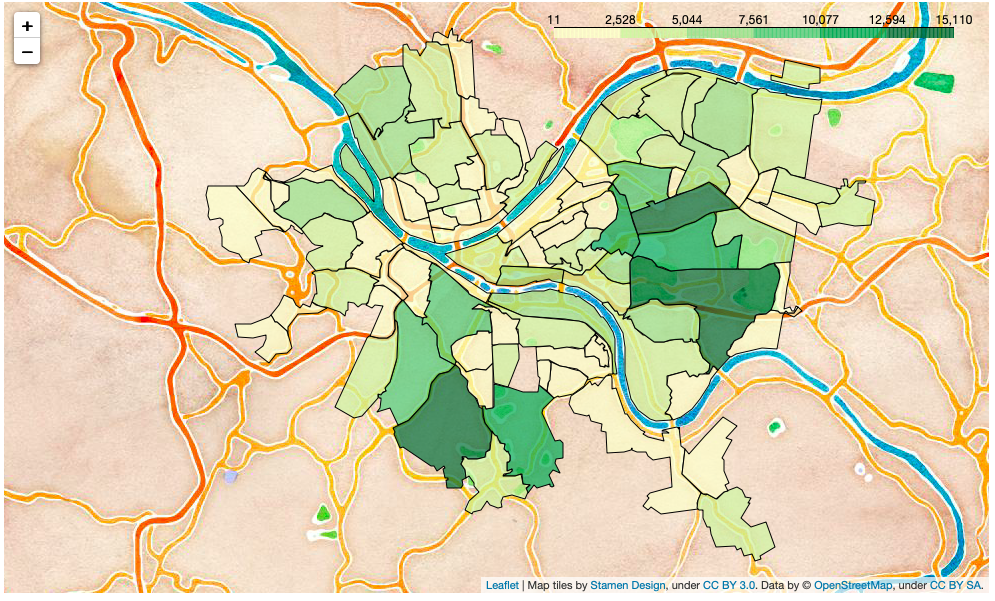
\includegraphics[scale=0.35]{popu.png}
\end{center}
As we can see from the graph.
The population of each neighborhood is mainly determined
by the area of the neighborhood.
It is usually the case the the larger the neighborhood is,
the more people live in it.

Therefore, to better understand the how crowded each neighborhood is,
we divided the population by the area of each neighborhood,
and visualize this population density.
\begin{center}
    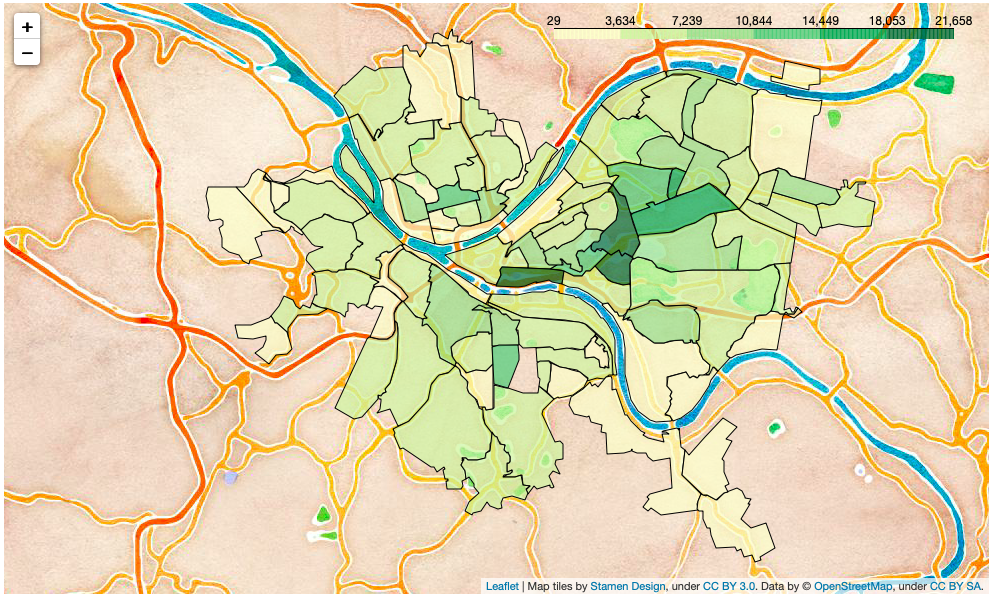
\includegraphics[scale=0.35]{popu_den.png}
\end{center}
As we can see from the plot, some of the most populated and crowded neighborhoods
are North Oakland, South Oakland, and Shadyside.

The next, we explore the job distribution in the city.
The following plot shows the number of jobs available
in each neighborhoods.
\begin{center}
    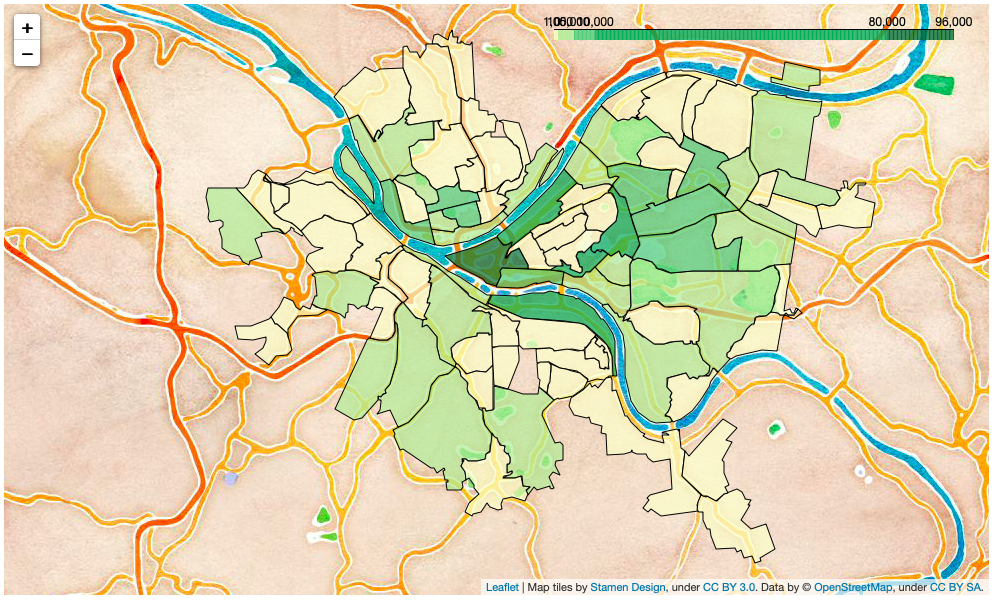
\includegraphics[scale=0.35]{job_distribution.png}
\end{center}
Clearly, there are most jobs in the Central Business District.
So, it would usually be more convenient to go to work,
if one lives closer to the Central Business District.

Using the Blotter of Police of Pittsburgh, we estimated
the frequentness of crimes in each neighborhoods using
the following metrics
\[monthly\_crime\_per\_person =
\frac{number\_of\_crimes\_in\_a\_month}{population\_of\_the\_neighborhood}\]
After calculating the average monthly crime per population for each
neighborhood, we plot it in the following graph:
\begin{center}
    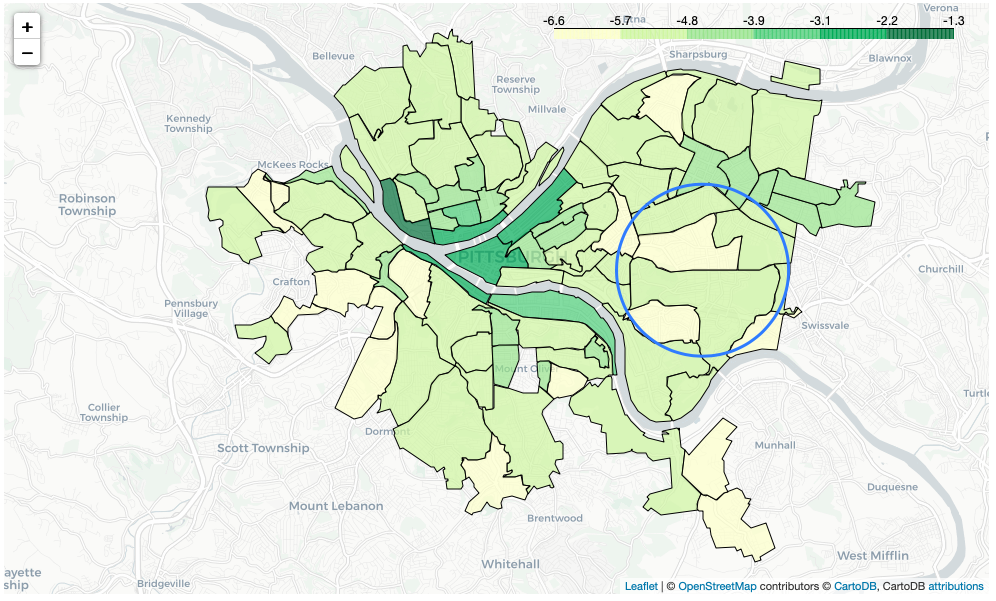
\includegraphics[scale=0.35]{crime.png}
\end{center}
As we can see, the are close to the CBD is where crime happens
most frequently, perhaps because it is the are where economic activities
happen most actively, and it is where people gather and communicate
most actively. Such area would not to be very nice for residence.
On the other hand, the circled area, which include Squirrel Hill North
actually has the lowest crime cases per person.
So, this neighborhood and the conjugate neighborhoods would be our
suitable candidates concerning safety and security.

We will settle down our choice of neighborhoods once
we look at the location of universities in Pittsburgh.
We listed the major universities in Pittsburgh in the following plot:
\begin{center}
    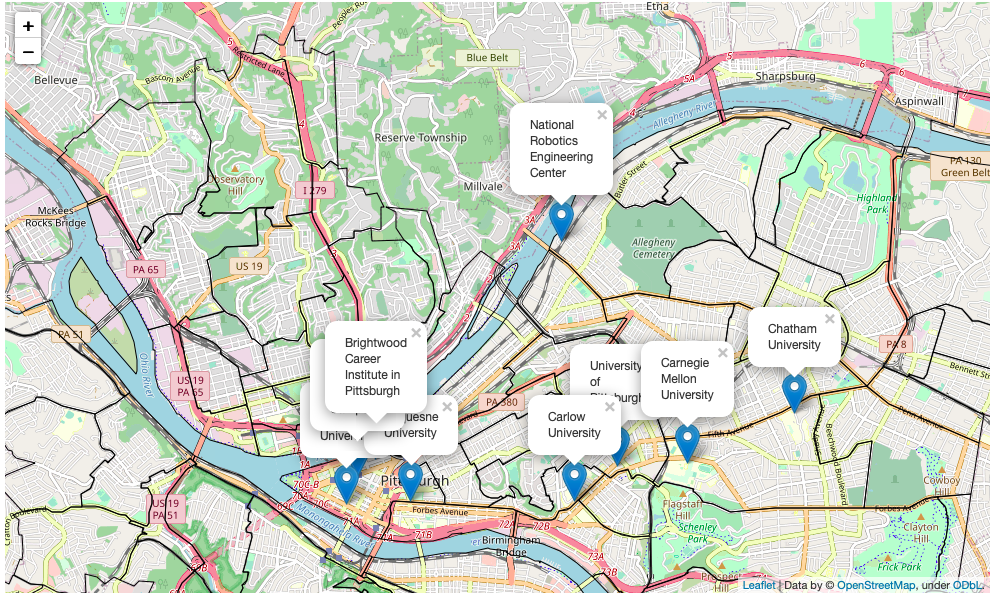
\includegraphics[scale=0.35]{univ.png}
\end{center}
Since, as we said, Jack wants to buy a house close to
universities. Considering the position of CMU and university of Pittsburgh,
we finally pin down the following neighborhoods as our candidates:
North Oakland, Shadyside, Squirrel Hill North, Squirrel Hill South,
Point Breeze, GreenField.

\subsection{Selecting Houses}
Having restricted our focus on North Oakland, Shadyside, Squirrel Hill North, Squirrel Hill South,
Point Breeze, GreenField, we now see which of the houses in these
areas have convenient public transit, and are close to supermarkets and hospitals.
Below is a plot of all the houses for us to choose from,
with the color indicating house prices (greener means cheaper, and redder means more expensive).
\begin{center}
    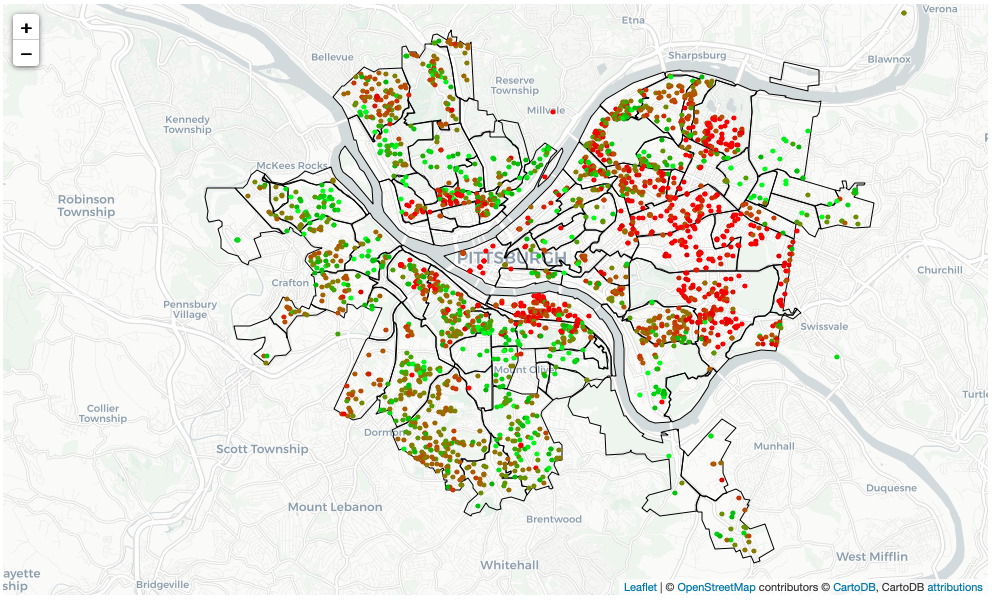
\includegraphics[scale=0.35]{houses.png}
\end{center}

Firstly, we try to figure out how many bus stations are there near
each of the houses.
Below is the distribution of the number of bus stations
within 500m for each of the houses:
\begin{center}
    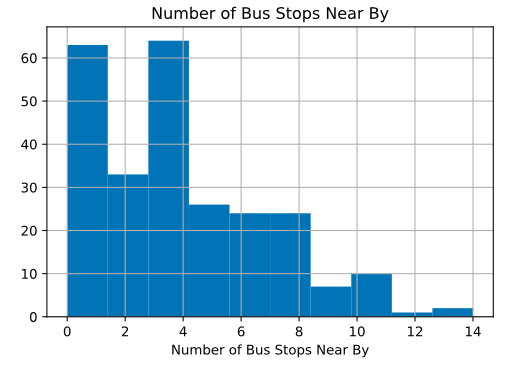
\includegraphics[scale=0.4]{bus.png}
\end{center}
We remove the houses which as only one bus station or no bus station
nearby (< 500m).

Then, we try to figure out how many supermarkets/malls are there near
each of the houses.
Below is the distribution of the number of supermarkets/malls
within 750m for each of the houses:
\begin{center}
    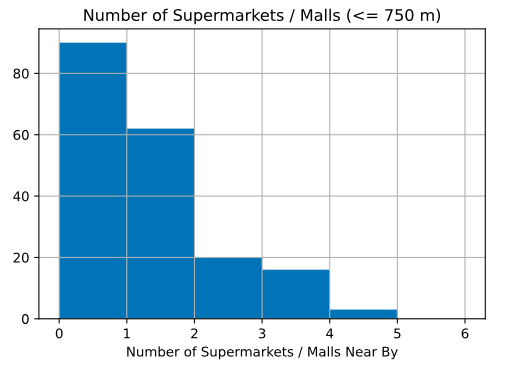
\includegraphics[scale=0.4]{mall.png}
\end{center}
We remove the houses which has no supermarket nearby (< 750m).

Thirdly, we try to figure out how many hospitals/doctor's offices are there near
each of the houses.
Below is the distribution of the number of hospitals/doctor's offices
within 750m for each of the houses:
\begin{center}
    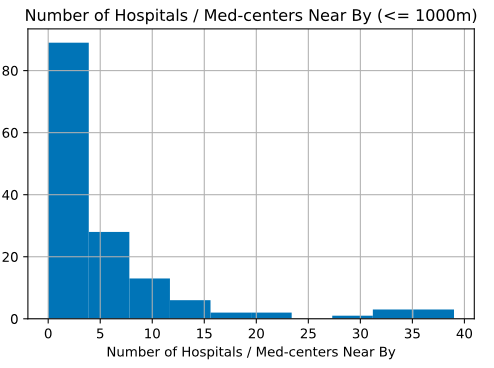
\includegraphics[scale=0.4]{med.png}
\end{center}
We remove the houses which has no hospital/doctor's office nearby (< 750m).

The houses left are plotted in the following map:
\begin{center}
    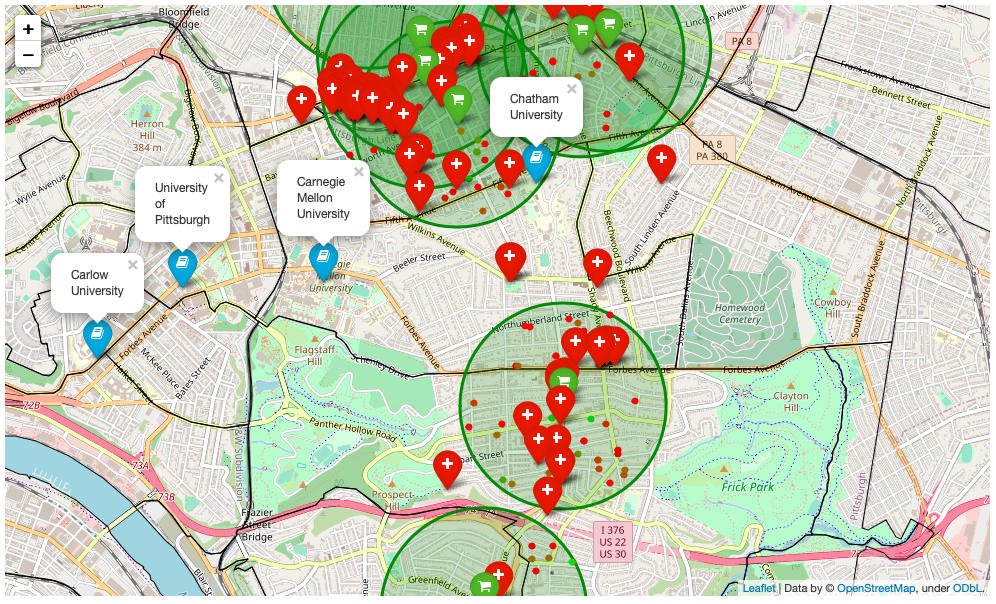
\includegraphics[scale=0.4]{restrict.png}
\end{center}

\subsection{Investment Opportunity}
Using the house sales data from Allegheny County Information Portal.
We estimated the median house prices of each of the neighborhoods.
We kept only valid and verified transactions for the purpose.

Regarding the neighborhoods of our choice, the estimation is summarized
in the following table.
\begin{center}
    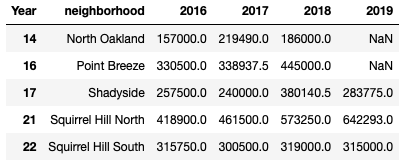
\includegraphics[scale=0.6]{median_price.png}
\end{center}
As we can see from the summary, the house prices of Squirrel Hill North
grows most steadily throughout 2016-2019,
compared to the data about other neighborhoods.
Therefore, we choose houses in Squirrel Hill North,
due to their good investment opportunity.

So, our final selection are the following fourteen houses
from Squirrel Hill North. We leave the final decision to Jack himself.
\begin{center}
    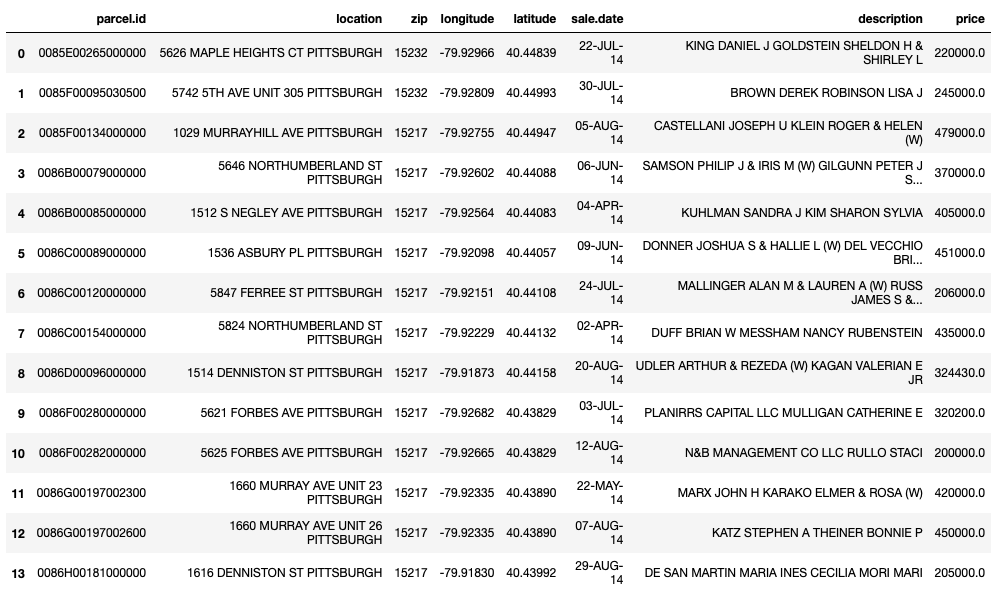
\includegraphics[scale=0.4]{result.png}
\end{center}

\section{Discussion}
Why don’t we narrow down the choices even more?
This is because we do not have information about Jack’s preference over house sizes,
decoration style, or his favorite entertainment and sports, etc.
There are still more to be taken into consideration only by Jack himself.

The data we use is sales-record over a year.
In cases when Jack really needs to buy a house,
there won’t be so many vacant houses to choose from.


\section{Conclusion}
Squirrel Hill North is nice, and has very good investment opportunity,
but it is not very convenient in terms of shopping.
It does not have a lot of supermarkets nearby.

Shadyside is a more mature community and has a lot of supermarkets there.
The downside of Shadyside is that it does not have as good an
investment potential as Squirrel Hill North.

Our final recommendation is still Squirrel Hill North.
It satisfy all the requirements and is the closest to major universities
compared to other neighborhoods.
It also most likely has a good investment potential.

\end{document}
